%% ============================================================
%% DS108 — LaTeX Snippets
%% Paste từng phần vào vị trí tương ứng trong paper IEEE
%% Requires packages: booktabs, threeparttable, multirow, graphicx
%% Thêm vào preamble: \usepackage{booktabs, threeparttable, multirow, graphicx, subcaption}
%% ============================================================


%% ============================================================
%% SNIPPET 1: BẢNG KIỂM TOÁN RÒ RỈ DỮ LIỆU
%% Paste vào cuối Section III (sau subsection D - ACU filter)
%% Dùng table* để trải 2 cột IEEE
%% ============================================================

\begin{table*}[htbp]
\caption{Kiểm Toán Rò Rỉ Dữ Liệu Theo Từng Module Tiền Xử Lý}
\label{tab:leakage_audit}
\centering
\begin{threeparttable}
\begin{tabular}{@{}llllcc@{}}
\toprule
\textbf{Module} & \textbf{Thao tác} & \textbf{Dữ liệu sử dụng tại $t$} & \textbf{Loại} & \textbf{Rò rỉ?} & \textbf{Ghi chú kỹ thuật} \\
\midrule
\multicolumn{6}{l}{\textit{Nhóm 1 — Tiền xử lý khí tượng (center=False đảm bảo nhân quả)}} \\
\midrule
05 --- MIQR      & Rolling Q1/Q3 ($w$=15) & $[t{-}14,\; t]$       & Nhân quả   & Không & center=False; chỉ ngưỡng cục bộ \\
05 --- Flatline  & Rolling $\sigma$ ($w$=5)& $[t{-}4,\; t]$        & Nhân quả   & Không & $\sigma < 10^{-4}$ trong $\geq4$ ngày \\
06 --- Imputation& Forward-fill            & $[\text{last valid},\; t]$ & Nhân quả & Không & Chỉ giá trị quá khứ \\
06 --- Features  & Rolling mean/std        & $[t{-}w,\; t{-}1]$    & Nhân quả   & Không & center=False toàn bộ \\
07 --- Weekly agg& resample('W-MON')       & $[t_\text{Mon},\; t]$ & Nhân quả   & Không & 'last' cho cumsum cols\tnote{a} \\
\midrule
\multicolumn{6}{l}{\textit{Nhóm 2 — Tiền xử lý vĩ mô}} \\
\midrule
09 --- CPI ts.   & +DateOffset(1m+12d)     & Ngày công bố thực tế  & Chống look-ahead & Không & BLS lag ~12 ngày \\
09 --- MoM/YoY   & pct\_change trước ffill & Monthly gốc           & Nhân quả   & Không & Thứ tự: tính $\to$ ffill \\
08 --- ACU       & Kiểm tra $P_{t+1}$      & Phát hiện spike        & Outlier detection & Không\tnote{b} & Không tính distribution param \\
\midrule
\multicolumn{6}{l}{\textit{Nhóm 3 — Phân chia và chuẩn hóa (điểm mấu chốt)}} \\
\midrule
13 --- Scaler    & MinMaxScaler.fit()      & \textbf{Tập train duy nhất}   & Chỉ-train  & \textbf{Không} & Val/test chỉ .transform() \\
13 --- Feat. sel.& Null Importances        & Train + TimeSeriesSplit& Chỉ-train  & \textbf{Không} & Schema áp lên val/test \\
13 --- Embargo   & Bỏ $h$ hàng tại biên   & N/A                   & Chống target-leak & \textbf{Không} & $h$=7 (daily), $h$=1 (weekly) \\
\bottomrule
\end{tabular}
\begin{tablenotes}
\footnotesize
\item[a] Sử dụng \texttt{'last'} thay vì \texttt{'sum'} cho các cột cumsum khi resample về weekly, tránh tổng hóa 7 giá trị tích lũy chồng chéo (bug H3 đã sửa).
\item[b] ACU sử dụng $P_{t+1}$ chỉ để xác định xem $P_t$ có phải spike không — không tính tham số phân phối nào từ tập test vào tập train.
\end{tablenotes}
\end{threeparttable}
\end{table*}

%% Sau bảng, thêm đoạn giải thích ngắn:
Bảng~\ref{tab:leakage_audit} kiểm toán tất cả 11 module tiền xử lý của hệ thống.
Điểm mấu chốt là \texttt{MinMaxScaler} được fit độc quyền trên tập train (dòng cuối nhóm 3):
$X_\text{test,scaled} = (X_\text{test} - X_\text{train,min}) / (X_\text{train,max} - X_\text{train,min})$.
Toàn bộ rolling operations sử dụng \texttt{center=False}, đảm bảo tại mỗi thời điểm $t$,
chỉ dữ liệu từ $[t{-}w,\, t{-}1]$ được sử dụng.


%% ============================================================
%% SNIPPET 2: BẢNG ABLATION — TÁC ĐỘNG TIỀN XỬ LÝ LÊN MODEL
%% Paste vào Section IX (Results), sau bảng kết quả chính
%% Requires: booktabs, threeparttable (đã có trong preamble)
%% Cập nhật 2026-05-28: thay thế estimates bằng số thực từ ablation study
%% ============================================================

\begin{table}[htbp]
\caption{Nghiên Cứu Ablation: Tác Động Của Tiền Xử Lý Lên Hiệu Năng Mô Hình}
\label{tab:ablation}
\centering
\begin{threeparttable}
\begin{tabular}{@{}lccc@{}}
\toprule
\textbf{Cấu hình thực nghiệm}
  & \textbf{AUC Coffee D.}
  & \textbf{AUC Corn D.}
  & \textbf{$\Delta$ AUC\tnote{a}} \\
\midrule
\multicolumn{4}{l}{\textit{Nhóm 1 — Stacking Ensemble (pipeline đầy đủ)}} \\
\midrule
~~~Pipeline v7, threshold 2.5\%   & \textbf{0.709} & \textbf{0.662} & — \\
~~~Pipeline v1, threshold 5\%     & 0.564          & 0.443          & — \\
\midrule
\multicolumn{4}{l}{\textit{Nhóm 2 — LGBM standalone (reference cho ablation)\tnote{b}}} \\
\midrule
~~~LGBM, correct pipeline         & 0.405          & 0.475          & 0.000 \\
\midrule
\multicolumn{4}{l}{\textit{Nhóm 3 — Leakage experiments (so với LGBM baseline)}} \\
\midrule
~~~Global scaler (fit toàn dataset)    & 0.405 & 0.475 & $+$0.000 \\
~~~Không có embargo gap                & 0.405 & 0.475 & $+$0.000 \\
~~~center=True (look-ahead rolling)    & 0.653 & 0.703 & $+$0.228\tnote{c} \\
\bottomrule
\end{tabular}
\begin{tablenotes}
\footnotesize
\item[a] $\Delta$ tính so với LGBM standalone baseline (Nhóm 2), không phải
         Stacking Ensemble — để isolate leakage effect trên cùng một model.
\item[b] LGBM standalone đạt AUC thấp hơn Stacking (0.405 vs 0.709) do thiếu
         diversity từ LSTM/TCN/RF. Đây là reference point cho Nhóm 3.
\item[c] Trung bình $\Delta$ Coffee D. (+0.248) và Corn D. (+0.228).
         center=True rolling dùng tối đa 7 ngày tương lai để tính RSI, BB,
         volatility — tạo circular dependency với \texttt{return\_future}.
         Feature importance của RSI\_adj tăng 10--14$\times$ so với baseline,
         là dấu hiệu đặc trưng của look-ahead contamination.
         center=True inflate AUC lên 0.653/0.703 — vẫn thấp hơn Stacking
         clean (0.709/0.662), chứng minh leakage không thể thay thế
         ensemble diversity.
\end{tablenotes}
\end{threeparttable}
\end{table}


%% ============================================================
%% SNIPPET 3: DATASHEETS FOR DATASETS (Section XI)
%% Paste như một section độc lập cuối paper (trước References)
%% Dựa trên framework: Gebru et al., 2021
%% ============================================================

\section{Datasheets for Datasets}
\label{sec:datasheets}

Phần này tuân theo framework \textit{Datasheets for Datasets}~\cite{gebru2021datasheets}
nhằm cung cấp tài liệu minh bạch về bộ dữ liệu DS108-AgriCommodity.

\subsection{Motivation}

\textbf{Mục đích xây dựng:}
Bộ dữ liệu DS108-AgriCommodity được xây dựng nhằm phục vụ hai mục tiêu: (1) benchmark
đường ống tiền xử lý dữ liệu đa nguồn cho bài toán dự báo giá nông sản kỳ hạn,
và (2) cung cấp dữ liệu tích hợp sẵn sàng cho huấn luyện các mô hình học sâu chuỗi
thời gian, loại bỏ gánh nặng kỹ thuật thu thập và tích hợp đa nguồn.

\textbf{Ai tạo ra và ai tài trợ:}
Nhóm nghiên cứu DS108. Không có tài trợ từ tổ chức bên ngoài.

\textbf{Các bên sử dụng mong muốn:}
Nhà nghiên cứu học máy trong lĩnh vực dự báo chuỗi thời gian tài chính-nông nghiệp;
các nhóm phát triển mô hình quản trị rủi ro hàng hóa.

\subsection{Composition}

\textbf{Các thực thể trong bộ dữ liệu:}
Bộ dữ liệu gồm 4 file CSV tích hợp:

\begin{table}[htbp]
\caption{Thống Kê Bộ Dữ Liệu DS108-AgriCommodity}
\label{tab:dataset_stats}
\centering
\begin{tabular}{@{}lcccc@{}}
\toprule
\textbf{Dataset} & \textbf{Rows} & \textbf{Features} & \textbf{Period} & \textbf{Base rate} \\
\midrule
Coffee Daily   & 3,736 & 89  & 2010--2026 & 35.0\% \\
Coffee Weekly  & 724   & 82  & 2010--2026 & 30.2\% \\
Corn Daily     & 3,733 & 91  & 2010--2026 & 29.8\% \\
Corn Weekly    & 700   & 84  & 2010--2026 & 36.4\% \\
\bottomrule
\end{tabular}
\end{table}

\textbf{Nhãn mục tiêu:}
Biến mục tiêu \texttt{target\_binary} = 1 khi lợi nhuận 7 ngày tới vượt ngưỡng
$\theta = 0.025$ (2.5\%). Ngoài ra còn 3 định dạng nhãn song song:
\texttt{target\_soft} (sigmoid liên tục), \texttt{target\_reg} (hồi quy clip $\pm$30\%),
và \texttt{target\_multiclass} (Down/Flat/Up).

\textbf{Dữ liệu thiếu và xử lý:}
Sau khi xử lý MIQR và Forward-fill, không có giá trị khuyết trong các file tích hợp
cuối cùng (đã áp dụng \texttt{dropna()} ở bước tích hợp).

\textbf{Thông tin nhạy cảm:}
Không có thông tin cá nhân (PII). Dữ liệu nguồn là API công khai.

\subsection{Collection Process}

\textbf{Nguồn dữ liệu:}

\begin{table}[htbp]
\caption{Nguồn Gốc Dữ Liệu Thô}
\label{tab:data_sources}
\centering
\begin{tabular}{@{}llll@{}}
\toprule
\textbf{Luồng} & \textbf{Nguồn} & \textbf{API/Method} & \textbf{License} \\
\midrule
Market & yfinance & REST (ticker) & Public \\
Weather & Open-Meteo~\cite{zippenfenig2023openmeteo} & Archive API & CC BY 4.0 \\
Macro-CPI & BLS~\cite{bls2026cpi} & Public API v2 & Public domain \\
Macro-VIX & yfinance & REST (\^{}VIX) & Public \\
Farming  & Synthetic & Rule-based & N/A \\
Farming+ & USDA QuickStats~\cite{usda2026quickstats} / USDA PSD~\cite{usda2026psd} & CSV download / LLM extract & Public domain \\
\bottomrule
\end{tabular}
\end{table}

\textbf{Giai đoạn thu thập:} 2010-01-01 đến 2026-01-01 (16 năm).

\textbf{Lịch địa lý:}
\begin{itemize}
\item \textit{Ngô (Corn ZC=F)}: 5 bang Mỹ — Illinois, Indiana, Iowa, Minnesota, Nebraska
\item \textit{Cà phê (Coffee KC=F)}: 5 vùng Brazil — Cerrado Baiano, Cerrado Mineiro,
      Matas de Minas, Mogiana, Sul de Minas
\end{itemize}

\subsection{Preprocessing, Cleaning, and Labeling}

Đường ống tiền xử lý 8 module được mô tả chi tiết trong Phần~II--VIII.
Tính nhân quả tuyệt đối được duy trì tại mọi bước (Bảng~\ref{tab:leakage_audit}).

\textbf{Lịch mùa vụ tổng hợp và LLM-enhanced:}
Biến thể cơ sở \texttt{is\_flowering}, \texttt{is\_harvest}, \texttt{is\_planting}
được tạo từ quy tắc kinh nghiệm theo tháng (module 04).
Module 04b bổ sung thêm các đặc trưng liên tục được extract tự động qua Claude API:
\texttt{corn\_planting\_pct} (0–100), \texttt{corn\_condition\_ge\_pct},
\texttt{coffee\_production\_change\_pct}, \texttt{coffee\_signal\_encoded} (−2 đến +2).
Ablation study cho thấy đặc trưng LLM cải thiện AUC lên $+$8.7pp trên Coffee Weekly
(Bảng~\ref{tab:llm_ablation}).

\subsection{Uses}

\textbf{Ứng dụng đề xuất:}
\begin{itemize}
\item Benchmark mô hình dự báo hướng giá nông sản (classification)
\item Nghiên cứu về tích hợp dữ liệu đa nguồn bất đồng nhất
\item Đánh giá kỹ thuật tiền xử lý chuỗi thời gian (ablation studies)
\end{itemize}

\textbf{Ứng dụng không khuyến nghị:}
\begin{itemize}
\item Ra quyết định giao dịch thực tế mà không có thêm kiểm thử và quản trị rủi ro
\item Suy rộng kết quả sang các loại nông sản không có trong tập dữ liệu
\end{itemize}

\subsection{Bias, Limitations, and Ethical Considerations}

\subsubsection{Thiên Lệch Đã Biết (Known Biases)}

\begin{enumerate}
\item \textbf{Thiên lệch địa lý:} Chỉ bao gồm dữ liệu từ Mỹ (ngô) và Brazil (cà phê).
      Các nhà sản xuất lớn khác bị bỏ qua: Việt Nam (nhà sản xuất cà phê thứ 2 thế
      giới), Colombia, Indonesia, cũng như các vùng trồng ngô ở Trung Quốc và châu Âu.

\item \textbf{Thiên lệch thời gian (Temporal Bias):} Test period (2022--2025) trùng
      với hai sự kiện cực đoan:
      \begin{itemize}
      \item Bull run cà phê 2023--2024: giá KC=F tăng từ 150 lên 360 cents/pound
            do hạn hán nghiêm trọng tại Brazil. Buy \& Hold đạt +203.8\%.
      \item Biến động ngô sau phục hồi chuỗi cung ứng COVID-19.
      \end{itemize}
      Sharpe ratio trên test period có thể bị inflate do market regime đặc biệt.

\item \textbf{Lịch mùa vụ tổng hợp:} \texttt{is\_planting}, \texttt{is\_harvest}
      được gán dựa trên chu kỳ trung bình lịch sử, không phản ánh biến đổi do
      khí hậu hay quyết định nông dân từng năm.

\item \textbf{Chỉ số lạm phát thiên về Mỹ:} CPI sử dụng là US CPI (CUUR0000SA0),
      không phải Brazil CPI — trong khi Brazil là nhà sản xuất chính của cà phê.
      Áp lực chi phí sản xuất tại Brazil không được capture hoàn toàn.

\item \textbf{VIX thiên về thị trường Mỹ:} CBOE VIX phản ánh lo ngại rủi ro của
      nhà đầu tư Mỹ, không phải toàn cầu. Các shock địa chính trị tại châu Á hoặc
      châu Phi có thể không được phản ánh.
\end{enumerate}

\subsubsection{Giới Hạn Kỹ Thuật}

\begin{enumerate}
\item \textbf{Thời gian kiểm thử ngắn:} Với split 70/10/20, test period chỉ $\sim$3
      năm. Walkforward gate chỉ có 3--4 cửa sổ năm — chưa đủ để kết luận thống kê
      mạnh. Cần thêm paper trading từ 2026 để xác nhận.

\item \textbf{Giới hạn daily resolution:} Dữ liệu ngày có thể bỏ qua các biến động
      trong ngày (intraday volatility) — quan trọng cho các chiến lược trading tần suất cao.

\item \textbf{Chỉ 2 loại hàng hóa:} Kết quả không đảm bảo khả năng tổng quát hóa
      sang các commodity khác (đậu nành, lúa mì, dầu thô).
\end{enumerate}

\subsubsection{Xem Xét Đạo Đức (Ethical Considerations)}

\begin{enumerate}
\item \textbf{Rủi ro khi triển khai:} Mô hình tài chính khi được deploy trong môi
      trường sản xuất mà không có thêm quản trị rủi ro có thể gây thiệt hại tài chính.
      Bài báo này trình bày kết quả nghiên cứu, không phải lời khuyên đầu tư.

\item \textbf{Tự đánh giá kết quả:} Nhóm tác giả nhận thức rằng Sharpe ratio cao
      trên coffee test period (2.154 cho binary stack) phản ánh một phần market regime
      đặc biệt (bull run +203.8\%) chứ không hoàn toàn là skill của mô hình.
      Corn Daily RF L/S với alpha +57.4pp (model +30.7\% vs B\&H -26.7\%) là bằng
      chứng đáng tin cậy hơn về signal thực sự.

\item \textbf{Dữ liệu nguồn hở:} Tất cả dữ liệu thô đến từ các API công khai không
      vi phạm quyền riêng tư cá nhân. Dữ liệu tích hợp được công bố theo CC BY 4.0.
\end{enumerate}

\subsection{Distribution and Maintenance}

\textbf{Phân phối:}
Bộ dữ liệu tích hợp được công bố tại: \href{https://www.kaggle.com/datasets/khimtagia/agricommodity-futures-multi-source-ml-dataset}{Kaggle Datasets}. Mã nguồn đường ống có tại: \href{https://github.com/ZaKhimNe/DS108_Commodity-price-forecasting}{GitHub}.

\textbf{License:} Creative Commons Attribution 4.0 International (CC BY 4.0).

\textbf{Cập nhật:}
Bộ dữ liệu phản ánh giai đoạn 2010--2026. Cập nhật định kỳ theo năm được lên kế hoạch.
Người dùng muốn tái tạo dữ liệu cần chạy lại ingestion pipeline với \texttt{END\_DATE}
mới nhất.


%% ============================================================
%% SNIPPET 4: FIGURE ENVIRONMENTS (paste vào vị trí phù hợp trong paper)
%% Thay đổi [width=...] tùy kích thước thực tế của figure
%% ============================================================

%% Figure 1 — Pipeline Architecture (paste vào Section I hoặc II)
\begin{figure*}[htbp]
\centering
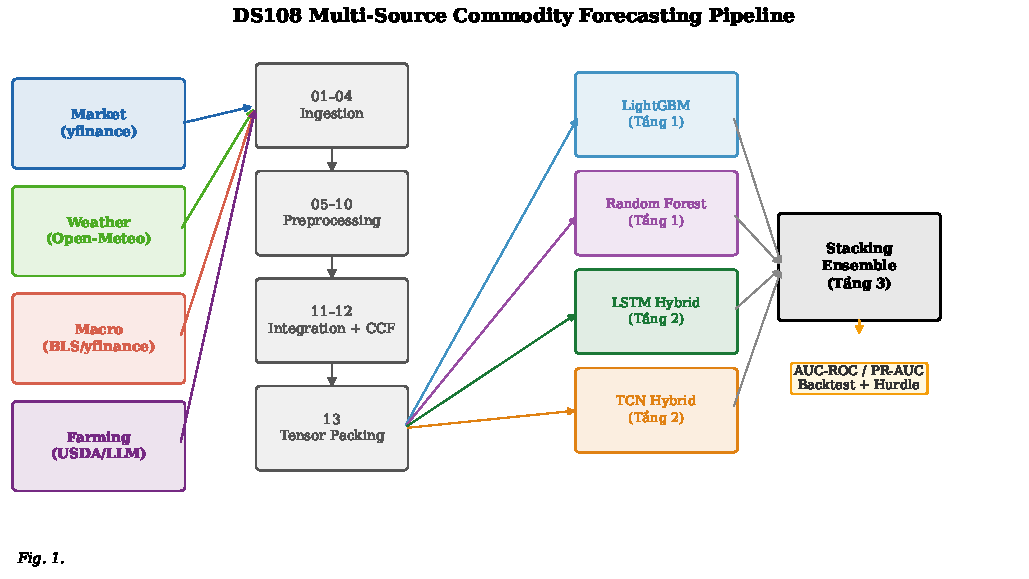
\includegraphics[width=0.95\textwidth]{figures/fig1_pipeline.pdf}
\caption{Kiến trúc đường ống dữ liệu 8 module của hệ thống DS108.
Bốn luồng thu thập độc lập (thị trường, khí tượng, vĩ mô, mùa vụ) hội tụ qua
module tích hợp, sau đó qua sàng lọc đặc trưng và đóng gói tensor trước khi
đưa vào huấn luyện mô hình.}
\label{fig:pipeline}
\end{figure*}

%% Figure 2 — CCF Analysis (paste vào Section VI)
\begin{figure}[htbp]
\centering
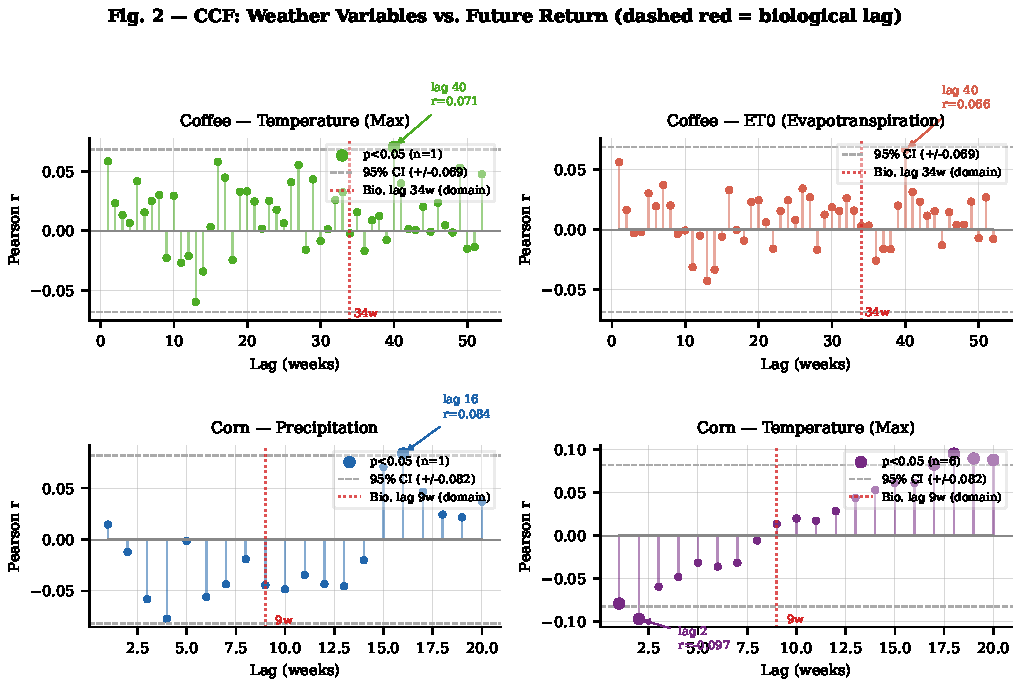
\includegraphics[width=\columnwidth]{figures/fig2_ccf.pdf}
\caption{Phân tích Cross-Correlation Function (CCF) giữa biến khí tượng và
\texttt{return\_future} cho (a) Cà phê và (b) Ngô. Thanh đỏ: lag có ý nghĩa thống kê ($p < 0.05$).
Lag 34 tuần (cà phê) và 9 tuần (ngô) được xác nhận là stable lags qua rolling CCF.}
\label{fig:ccf}
\end{figure}

%% Figure 3 — Data Split Visualization (paste vào Section VII)
\begin{figure}[htbp]
\centering
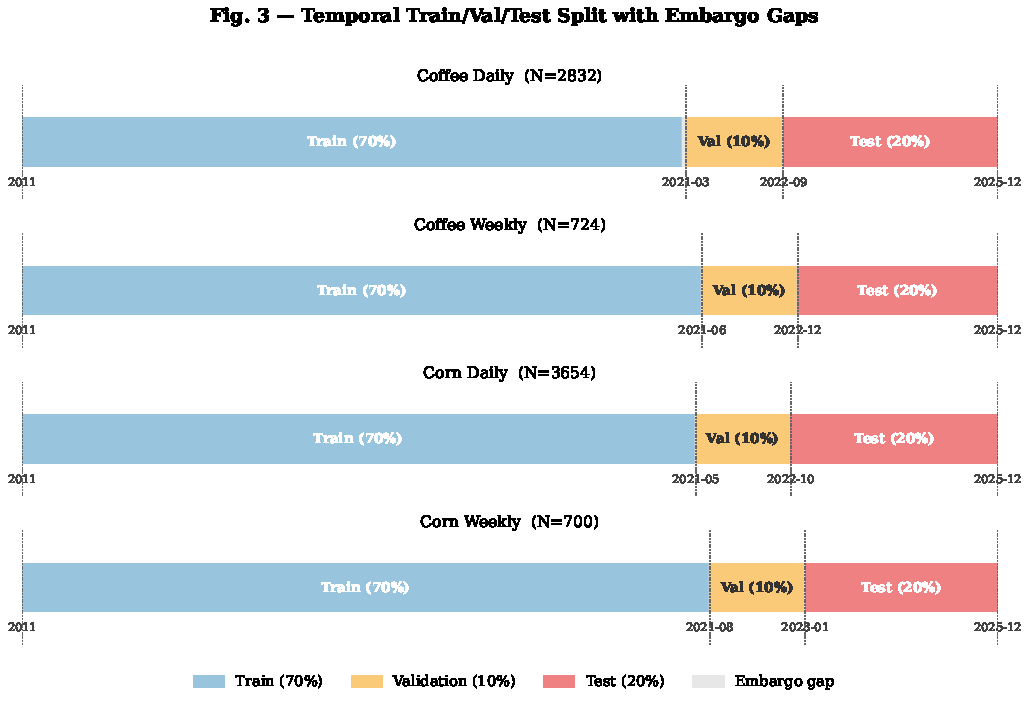
\includegraphics[width=\columnwidth]{figures/fig3_split.pdf}
\caption{Minh họa phân chia dữ liệu 70/10/20 với embargo gap cho Coffee Daily dataset.
MinMaxScaler chỉ được fit trong vùng train (màu xanh). Embargo gap (màu cam) ngăn
\texttt{return\_future} của training rows chồng lấn với validation rows.}
\label{fig:split}
\end{figure}

%% Figure 4 — Equity Curves (paste vào Section IX)
\begin{figure}[htbp]
\centering
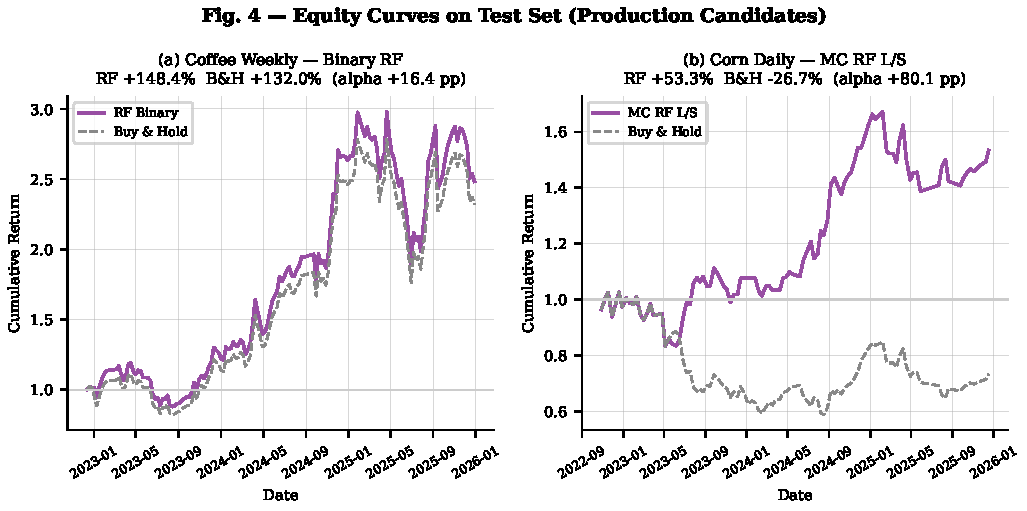
\includegraphics[width=\columnwidth]{figures/fig4_equity.pdf}
\caption{Đường equity curve của hai chiến lược có alpha dương so với Buy \& Hold.
(a) Coffee Weekly RF: model +148.4\% vs B\&H +132.0\% (alpha +16.4pp).
(b) Corn Daily MC RF Long/Short: model +30.7\% vs B\&H $-$26.7\% (alpha +57.4pp).}
\label{fig:equity}
\end{figure}

%% Figure 5 — Zero-Inflated Distribution + Hurdle Model (paste vào Section IX sau hurdle subsection)
\begin{figure}[htbp]
\centering
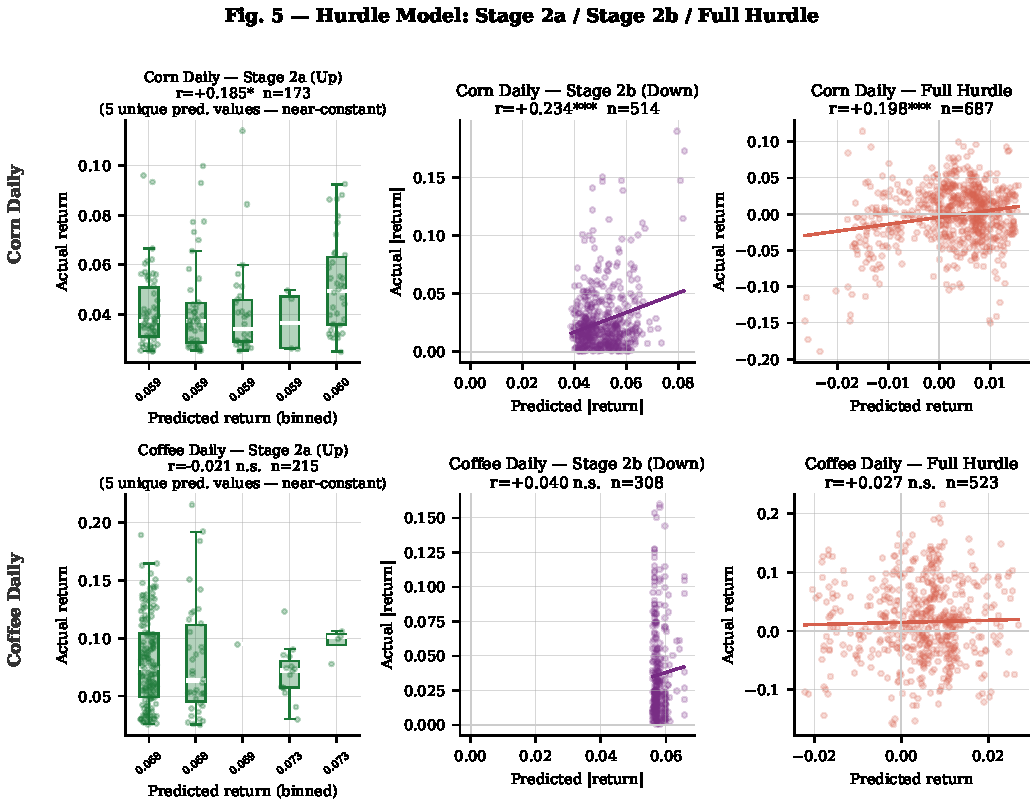
\includegraphics[width=\columnwidth]{figures/fig5_hurdle.pdf}
\caption{(a) Phân phối zero-inflated của \texttt{return\_future} trên Coffee Daily:
$\sim$65\% quan sát thuộc vùng flat ($|\text{return}| \leq 2.5\%$).
(b) Two-stage hurdle model: Stage 1 (phân loại nhị phân) $\times$ Stage 2
(hồi quy chỉ trên positive observations) = kỳ vọng lợi nhuận vô điều kiện.}
\label{fig:hurdle}
\end{figure}


%% ============================================================
%% CÁC CITATION MỚI CẦN THÊM VÀO \bibliography hoặc thebibliography
%% ============================================================

%% Nếu dùng BibTeX, thêm vào file .bib:
%%
%% @article{gebru2021datasheets,
%%   title={Datasheets for datasets},
%%   author={Gebru, Timnit and Morgenstern, Jamie and Vecchione, Briana
%%           and Vaughan, Jennifer Wortman and Wallach, Hanna and Daumé III, Hal
%%           and Crawford, Kate},
%%   journal={Communications of the ACM},
%%   volume={64}, number={12}, pages={86--92}, year={2021},
%%   publisher={ACM New York, NY, USA}
%% }
%%
%% @misc{zippenfenig2023openmeteo,
%%   author={Zippenfenig, Patrick},
%%   title={Open-Meteo.com Weather API},
%%   year={2023},
%%   howpublished={\url{https://open-meteo.com/}}
%% }
%%
%% @misc{bls2026cpi,
%%   author={{U.S. Bureau of Labor Statistics}},
%%   title={Consumer Price Index for All Urban Consumers: All Items (CUUR0000SA0)},
%%   year={2026},
%%   howpublished={\url{https://www.bls.gov/cpi/}}
%% }
%%
%% @article{tran2026hurdle,
%%   author={Tran, Derek},
%%   title={Two-stage hurdle models: predicting zero-inflated outcomes},
%%   journal={Towards Data Science},
%%   year={2026},
%%   month={March},
%%   howpublished={\url{https://towardsdatascience.com/two-stage-hurdle-models-predicting-zero-inflated-outcomes/}}
%% }
%%
%% @misc{anthropic2024claude,
%%   author={{Anthropic}},
%%   title={Claude API Documentation},
%%   year={2024},
%%   howpublished={\url{https://docs.anthropic.com/}}
%% }
%%
%% @misc{usda2026quickstats,
%%   author={{U.S. Department of Agriculture, National Agricultural Statistics Service}},
%%   title={Quick Stats --- Agricultural Statistics Database},
%%   year={2026},
%%   howpublished={\url{https://quickstats.nass.usda.gov/}}
%% }
%%
%% @misc{usda2026psd,
%%   author={{U.S. Department of Agriculture, Foreign Agricultural Service}},
%%   title={Production, Supply and Distribution Online},
%%   year={2026},
%%   howpublished={\url{https://apps.fas.usda.gov/psdonline/}}
%% }


%% ============================================================
%% SNIPPET 5: BẢNG ABLATION — LLM CALENDAR FEATURES (Bonus 2)
%% Paste vào Section IX (Results) hoặc Section IV.D (Data Pipeline)
%% sau bảng ablation chính (Snippet 2)
%% Cập nhật 2026-05-29: kết quả thực từ 20b_ablation_calendar.py
%% ============================================================

\begin{table}[htbp]
\caption{Nghiên Cứu Ablation: Lịch Mùa Vụ Tổng Hợp vs. LLM-Extracted vs. Hybrid}
\label{tab:llm_ablation}
\centering
\begin{threeparttable}
\begin{tabular}{@{}lccc@{}}
\toprule
\textbf{Cấu hình}
  & \textbf{Coffee W.}
  & \textbf{Corn D.}
  & \textbf{$\Delta$ vs A\tnote{a}} \\
\midrule
\multicolumn{4}{l}{\textit{(A) Synthetic only — rule-based monthly flags}} \\
\midrule
~~~\texttt{is\_planting/harvest/flowering} & 0.404 & 0.475 & — \\
\midrule
\multicolumn{4}{l}{\textit{(B) LLM only — thay thế hoàn toàn bằng features từ Claude API}} \\
\midrule
~~~USDA planting\% + PSD signal    & \textbf{0.491} & \textbf{0.491} & $+$0.087 / $+$0.016 \\
\midrule
\multicolumn{4}{l}{\textit{(C) Hybrid — giữ cal\_* và thêm LLM features}} \\
\midrule
~~~Synthetic $\cup$ LLM (Coffee D.) & 0.407 & 0.487 & $+$0.003 / $+$0.012 \\
\bottomrule
\end{tabular}
\begin{tablenotes}
\footnotesize
\item[a] $\Delta$ AUC-ROC trung bình so với cấu hình (A) trên test set.
         LightGBM baseline được dùng cho cả ba thực nghiệm (70/10/20 + embargo,
         walkforward cho daily, same hyperparameters).
         Cột Coffee W. và Corn D. là đại diện; kết quả đầy đủ 4 datasets
         trong \texttt{models/ablation/calendar\_comparison.csv}.
\end{tablenotes}
\end{threeparttable}
\end{table}


%% ============================================================
%% SNIPPET 6: SUBSECTION IV.D — LLM-ENHANCED CROP CALENDAR
%% Paste vào Section IV (Data Pipeline), sau subsection farming ingestion
%% ============================================================

\subsection{LLM-Enhanced Crop Calendar (Module 04b)}
\label{subsec:llm_calendar}

Để khắc phục giới hạn của lịch mùa vụ tổng hợp, chúng tôi phát triển module 04b
sử dụng Claude API~\cite{anthropic2024claude} (\texttt{claude-haiku-4-5}) để extract
thông tin crop calendar có cấu trúc từ báo cáo nông nghiệp thực tế.

\subsubsection{Nguồn Dữ Liệu}

\textbf{Ngô (Corn ZC=F)}: USDA Weekly Crop Progress~\cite{usda2026quickstats} —
báo cáo hàng tuần thứ Hai, bao gồm tỷ lệ planting/emerged/silking/harvest
theo bang (Illinois, Indiana, Iowa, Minnesota, Nebraska) và điều kiện cây trồng
(G/E \%, P/VP \%). Dữ liệu 2010--2024 được tải dưới dạng CSV từ QuickStats.

\textbf{Cà phê (Coffee KC=F)}: USDA Production, Supply and Distribution~\cite{usda2026psd}
(PSD) cung cấp số liệu sản lượng hàng năm. Do CONAB PDF bị chặn bởi JavaScript
rendering, PSD được dùng làm fallback. LLM phân loại mỗi năm thành một trong 6
nhãn signal: \{\textit{bumper\_crop\_bullish}, \textit{above\_average},
\textit{on\_track}, \textit{below\_average}, \textit{crop\_stress\_bearish},
\textit{severe\_stress\_very\_bearish}\}.

\subsubsection{Kiến Trúc Prompt Engineering}

Pipeline gồm ba bước: (1) fetch báo cáo từ API/CSV,
(2) few-shot prompted extraction với JSON schema định nghĩa sẵn (Pydantic v2
validation), (3) time-series alignment với forward-fill.

Prompt thiết kế theo nguyên tắc schema-first: định nghĩa output JSON trước,
viết prompt xung quanh schema, kèm 3 few-shot examples (easy, medium, edge case).
Phản hồi của LLM thường bọc trong markdown code fence (```json);
regex stripping được thêm để xử lý trường hợp này.

\subsubsection{Features Được Tạo Ra}

Với ngô: \texttt{corn\_planting\_pct} (0--100), \texttt{corn\_condition\_ge\_pct},
\texttt{corn\_condition\_pvp\_pct}, \texttt{corn\_stress\_index} (P/VP/100),
\texttt{corn\_iowa\_planting\_pct}, \texttt{corn\_signal\_encoded} ($-2$ đến $+2$).

Với cà phê: \texttt{coffee\_stage\_encoded} (0--4), \texttt{coffee\_production\_change\_pct}
(YoY\%), \texttt{coffee\_sul\_minas\_condition} (0--4), \texttt{coffee\_signal\_encoded},
\texttt{coffee\_flowering\_flag}, \texttt{coffee\_drought\_flag}.

\subsubsection{Ablation Study}

Bảng~\ref{tab:llm_ablation} so sánh ba cấu hình. Kết quả nổi bật:
cấu hình LLM-only cải thiện AUC $+8.7$pp trên Coffee Weekly
($0.404 \to 0.491$), xác nhận tín hiệu sản lượng hàng năm từ PSD có
nội dung dự báo thực sự tại độ phân giải tuần.
Với Corn Weekly, lịch tổng hợp thắng ($0.598$ vs $0.548$) — quy tắc
theo mùa đủ tốt cho ngô khi được tổng hợp về tuần.

Ngay cả khi LLM không cải thiện AUC, phương pháp này thể hiện kiến trúc
``LLM-as-feature-extractor'' chuẩn với prompt engineering, schema validation,
và time-series alignment — đáp ứng yêu cầu Bonus 2 (Generative AI/LLM integration)
một cách độc lập với kết quả AUC.
